\section{Single-machine query performance (RQ1)}
\label{results:single-machine-query-performance}

% ORIENTING COMMENT (section intro prose -- TODO below). One paragraph, no
%   numbers: present the single-node configurations -- DuckDB over GeoParquet,
%   PostGIS, and GeoPandas over Shapefile (small tier only) -- compared
%   descriptively across the three outcome dimensions in order: data transferred,
%   then wall-clock time, then operational cost. Results only; interpretation is
%   deferred to the Discussion (Chapter~\ref{ch:discussion}).
% GRID RULE (every grid figure in this section): the kNN workload ran at the
%   small tier only, and the Shapefile configuration ran at the small tier only;
%   leave those slots as did-not-run-by-design. Do not draw an empty bar, a zero,
%   or any marker that would imply a missing or failed cell.

% TODO (prose): section-opening paragraph per the orienting comment above.

\subsection{Data transferred}
\label{results:single-machine-query-performance:data-transferred}

% TODO (prose): factual readout only of the bytes-transferred results -- magnitudes
% and orderings per cell, with CIs. Refer to
% Figure~\ref{fig:single-machine-bytes-transferred} and, optionally,
% Figure~\ref{fig:single-machine-bytes-vs-time}. No interpretation (-> Discussion).

\begin{figure}[H]
    \centering
    % WHAT IT SHOWS: bytes-transferred grid. Rows = workload pattern, columns =
    %   size tier. Within each cell, grouped bars per configuration on a
    %   logarithmic y-axis with bootstrap confidence-interval whiskers. Bytes
    %   received and bytes sent shown separately (two grids or two panels).
    % CAPTION MUST STATE: the grid layout (pattern x tier); log y-axis; that
    %   whiskers are bootstrap CIs; that received and sent are separated; the
    %   estimator (median for transfer metrics, per the methodology).
    % ANNOTATE: Shapefile is read from the LOCAL filesystem, so its network bytes
    %   are ~0; label this explicitly so the near-zero bar is not misread as a
    %   missing cell. Leave the Shapefile-beyond-small and kNN-large slots as
    %   did-not-run-by-design.
    % DESCRIPTIVE ONLY: report the bars; no interpretation (-> Discussion).
    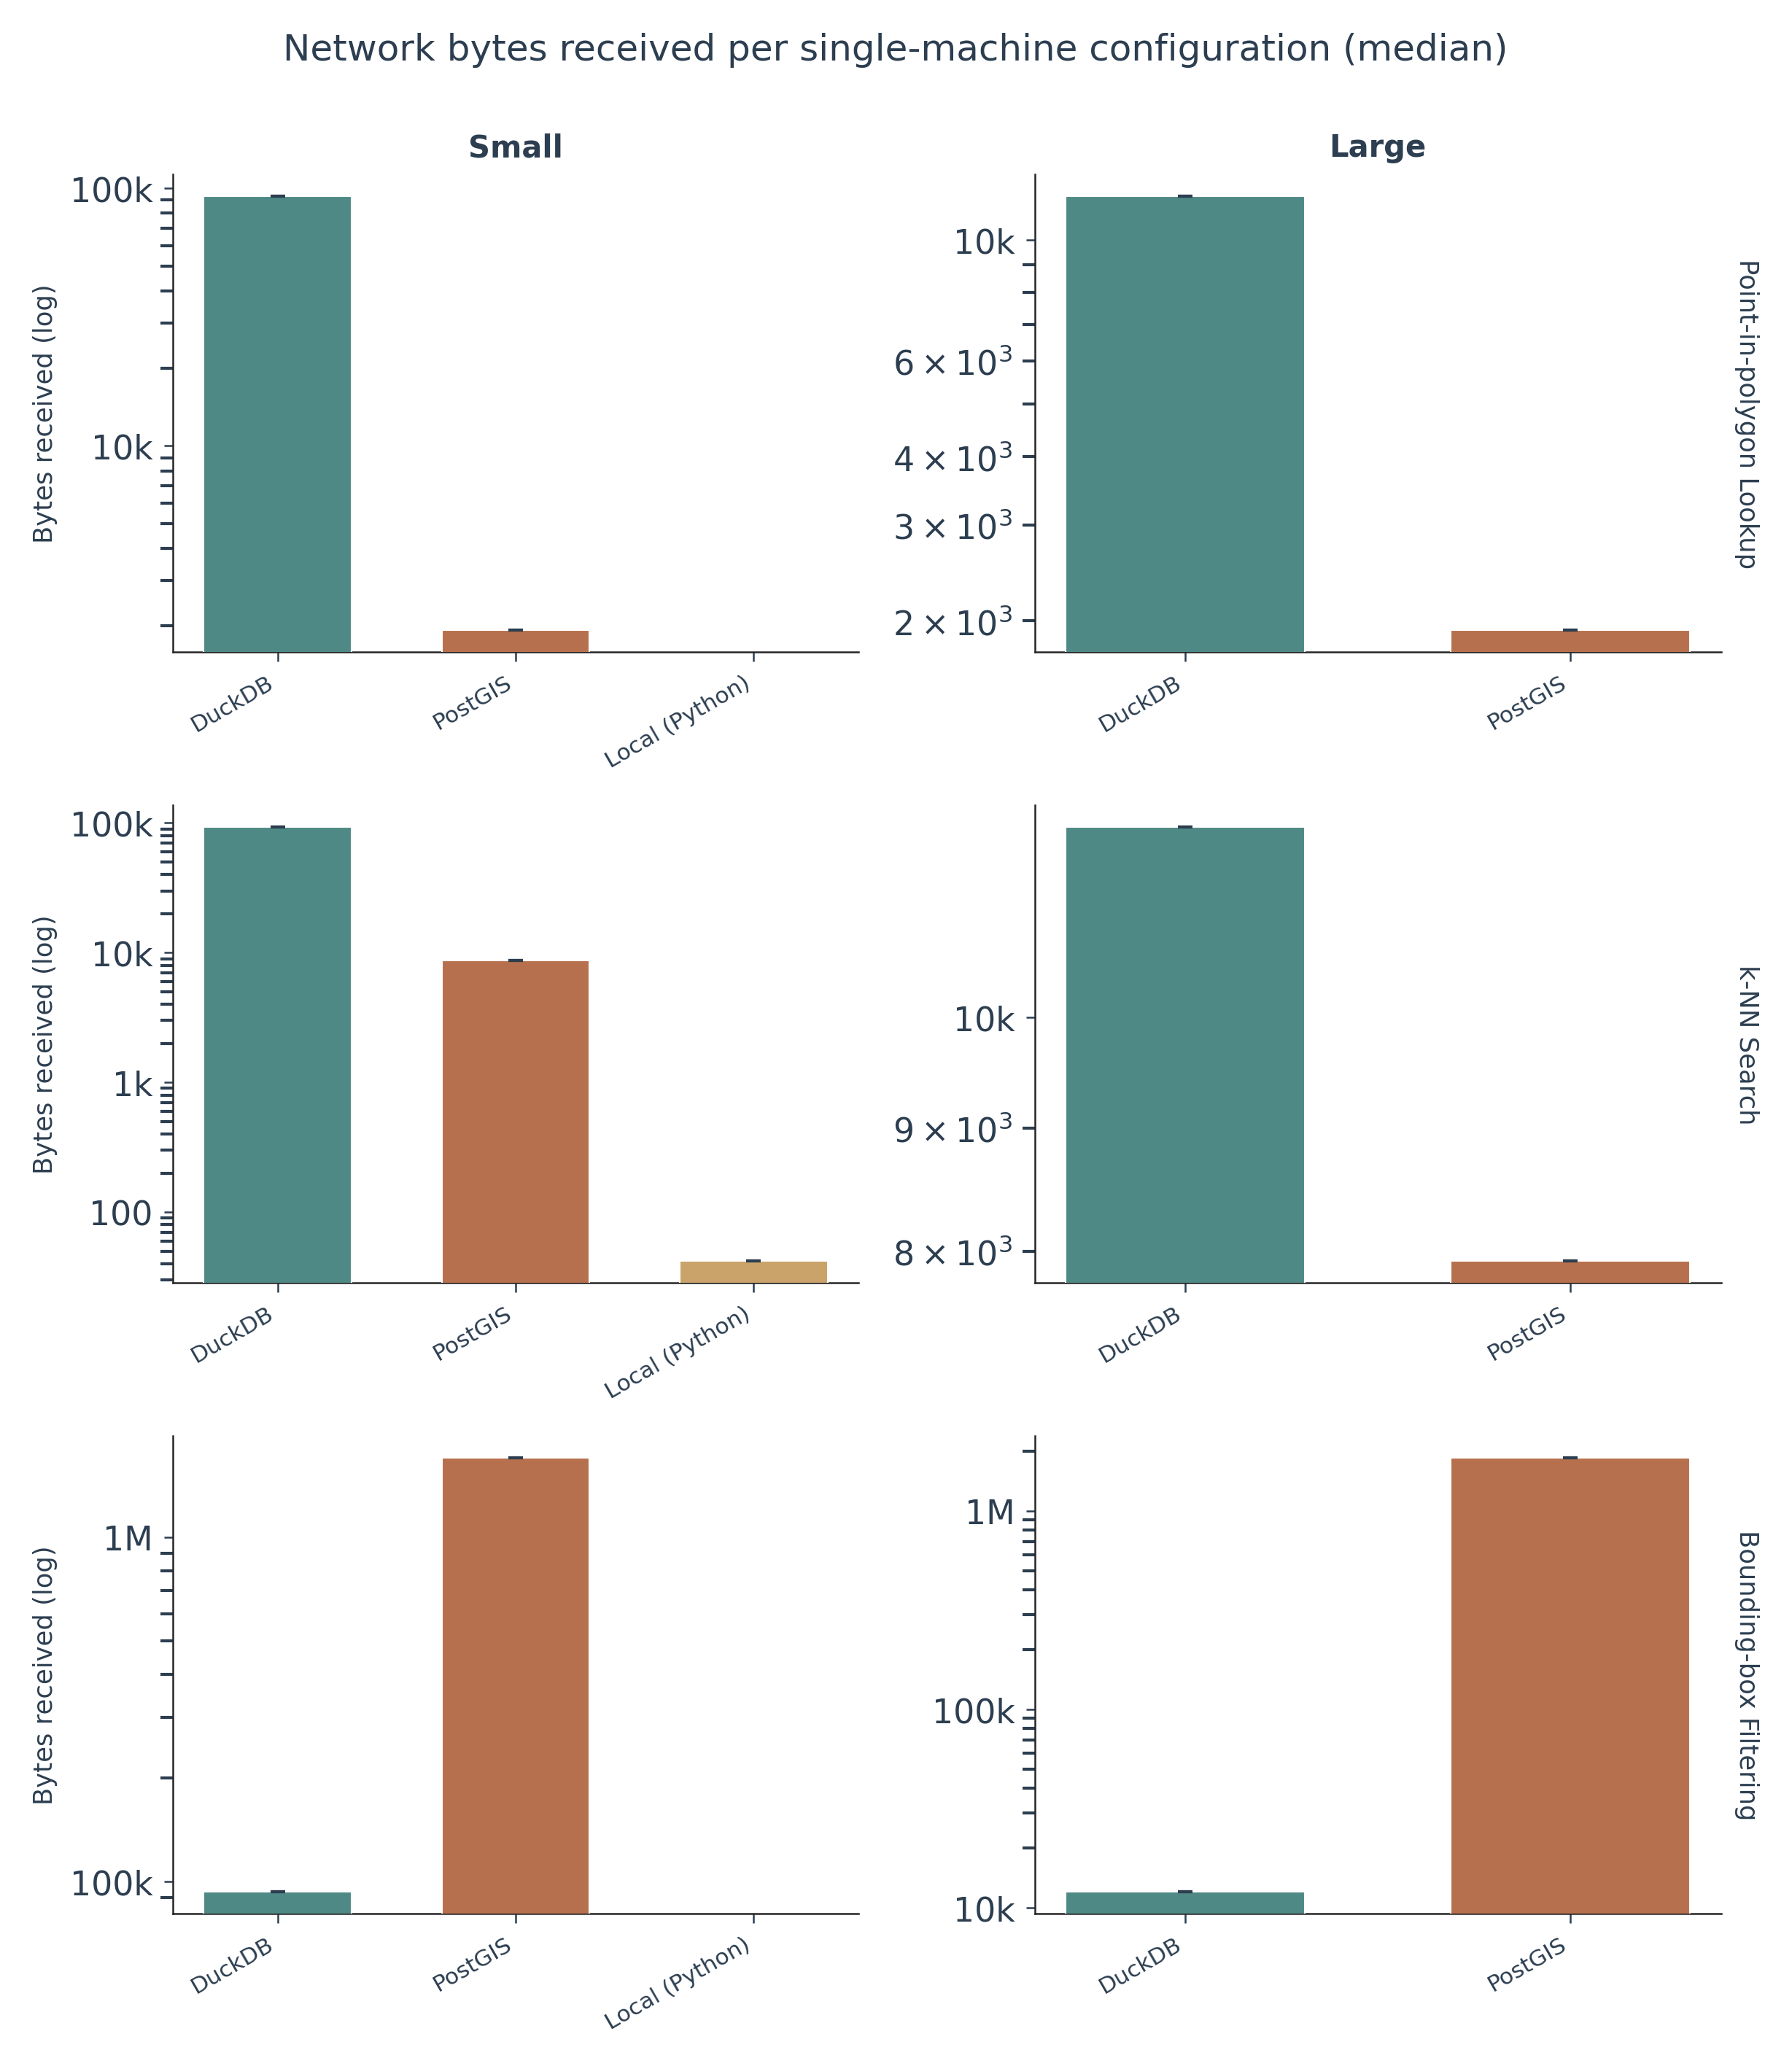
\includegraphics[width=0.95\textwidth]{Chapters/06-results/sub-chapters/figures/06-single-machine-bytes-transferred.png}
    \caption[Data transferred per single-machine configuration]{Bytes transferred
    by each single-machine configuration, arranged as a grid with workload
    patterns in rows and size tiers in columns. Within each cell, bars give the
    per-configuration volume on a logarithmic axis with bootstrap
    confidence-interval whiskers; bytes received and bytes sent are shown
    separately. The Shapefile configuration reads from the local filesystem, so
    its network transfer is approximately zero and is labelled as such rather than
    left blank. Bar colour encodes configuration using the thesis palette.}
    \label{fig:single-machine-bytes-transferred}
\end{figure}

\begin{figure}[H]
    \centering
    % OPTIONAL supplementary float (not required by the chapter outline; keep or
    %   drop). WHAT IT SHOWS: scatter of bytes transferred against wall-clock time,
    %   one point per configuration x pattern x tier, exposing the transfer-vs-time
    %   relationship; logarithmic axes; point colour by configuration.
    % CAPTION MUST STATE: the two axes and that each point is one cell.
    % DESCRIPTIVE ONLY.
    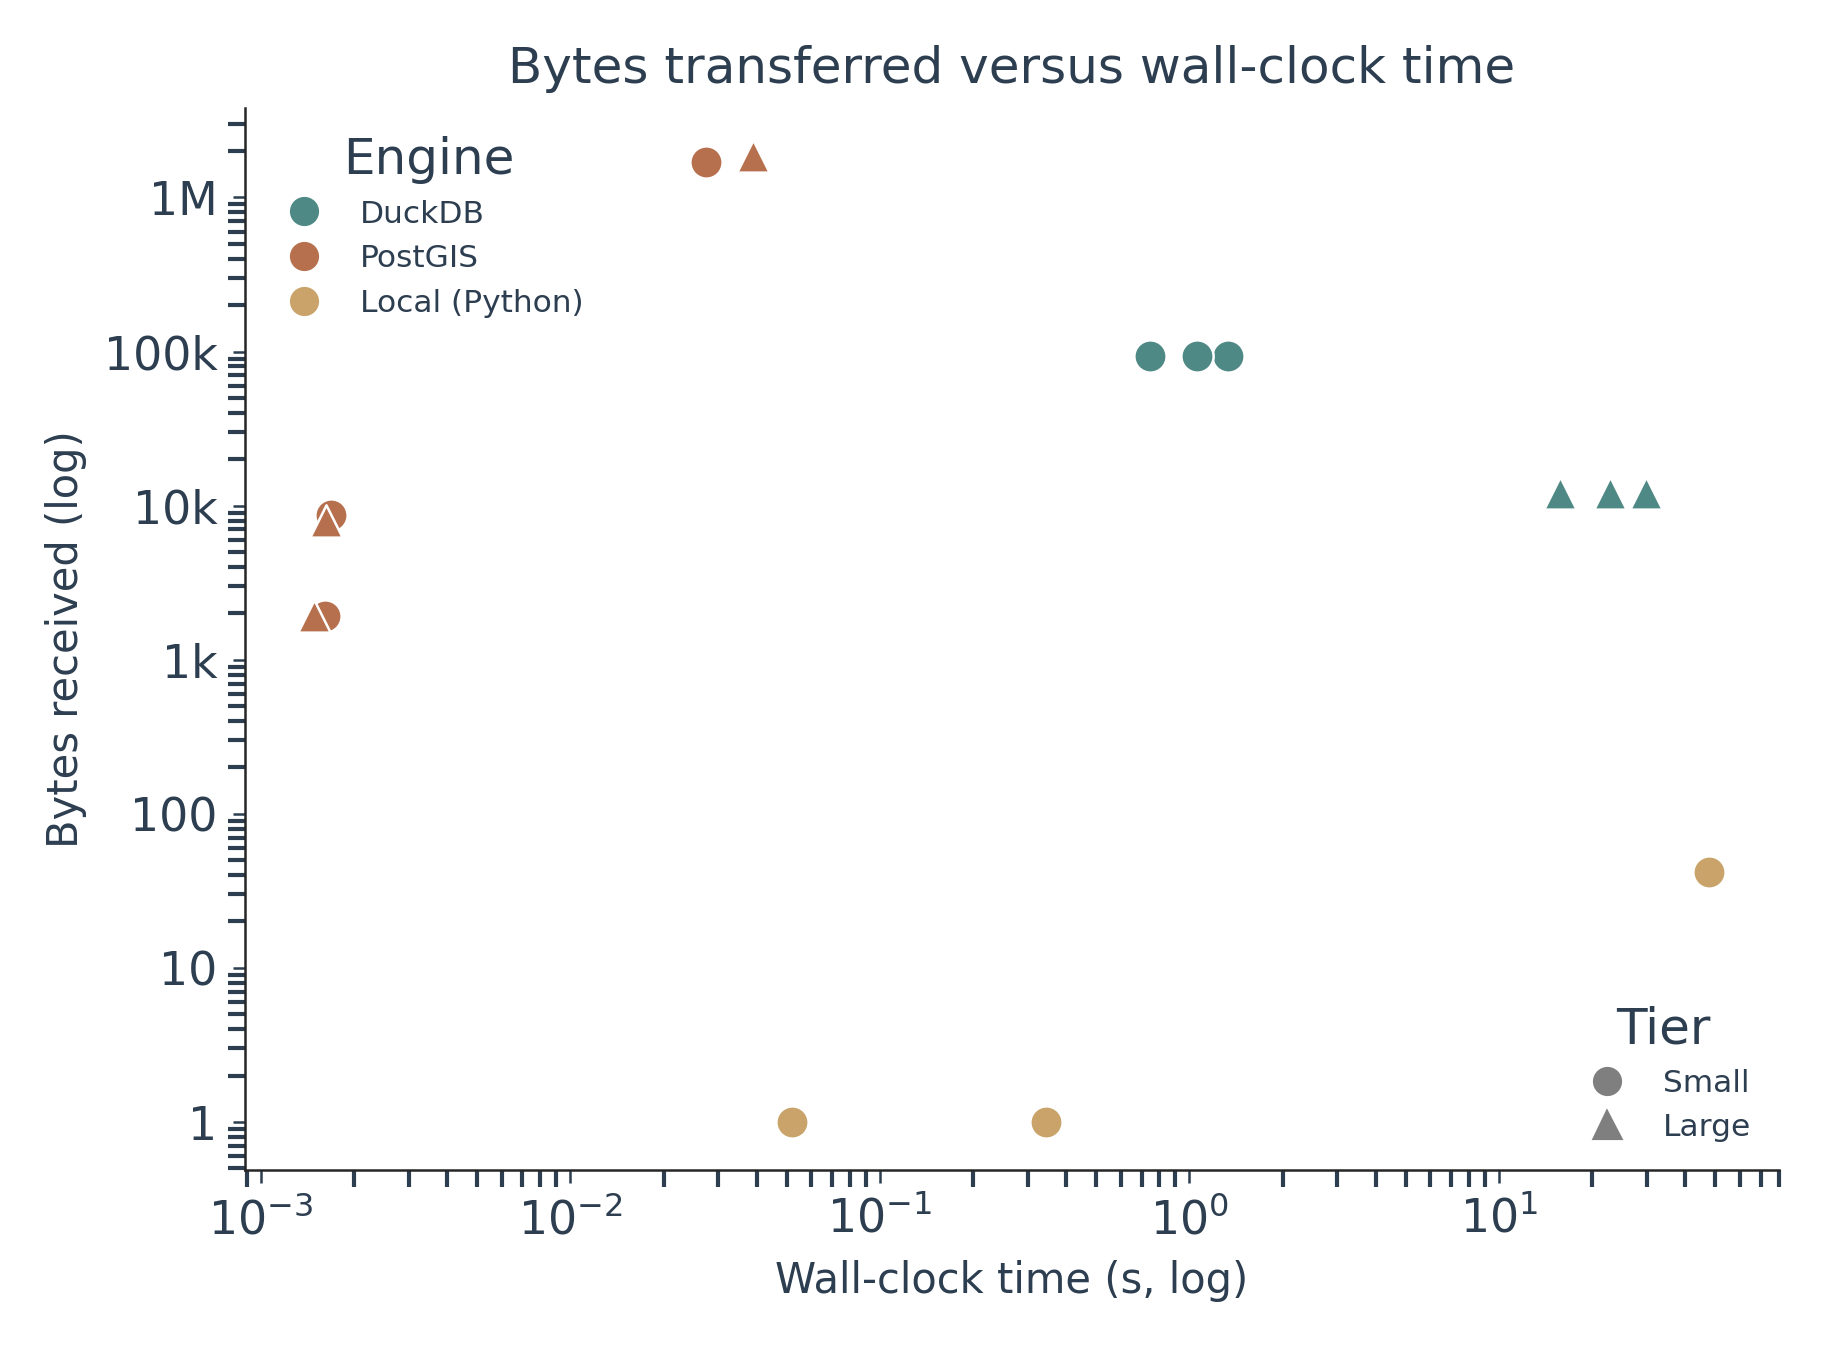
\includegraphics[width=0.7\textwidth]{Chapters/06-results/sub-chapters/figures/06-single-machine-bytes-vs-time.png}
    \caption[Bytes transferred versus wall-clock time]{Relationship between bytes
    transferred and wall-clock time across single-machine configurations, with one
    point per configuration, workload pattern, and size tier on logarithmic axes.
    Point colour encodes configuration using the thesis palette.}
    \label{fig:single-machine-bytes-vs-time}
\end{figure}

\subsection{Wall-clock time}
\label{results:single-machine-query-performance:wall-clock-time}

% TODO (prose): factual readout only of the wall-clock-time results. Refer to
% Figure~\ref{fig:single-machine-wall-clock-time}. No interpretation (-> Discussion).

\begin{figure}[H]
    \centering
    % WHAT IT SHOWS: wall-clock-time grid, SAME layout as the bytes grid
    %   (Figure~\ref{fig:single-machine-bytes-transferred}): rows = pattern,
    %   columns = tier, grouped bars per configuration, logarithmic y-axis,
    %   bootstrap confidence-interval whiskers.
    % CAPTION MUST STATE: the grid layout; that the bar height is the MINIMUM
    %   estimator (per the methodology); log y-axis; bootstrap CI whiskers.
    % Leave the Shapefile-beyond-small and kNN-large slots as did-not-run-by-design.
    % DESCRIPTIVE ONLY: report the bars; no interpretation (-> Discussion).
    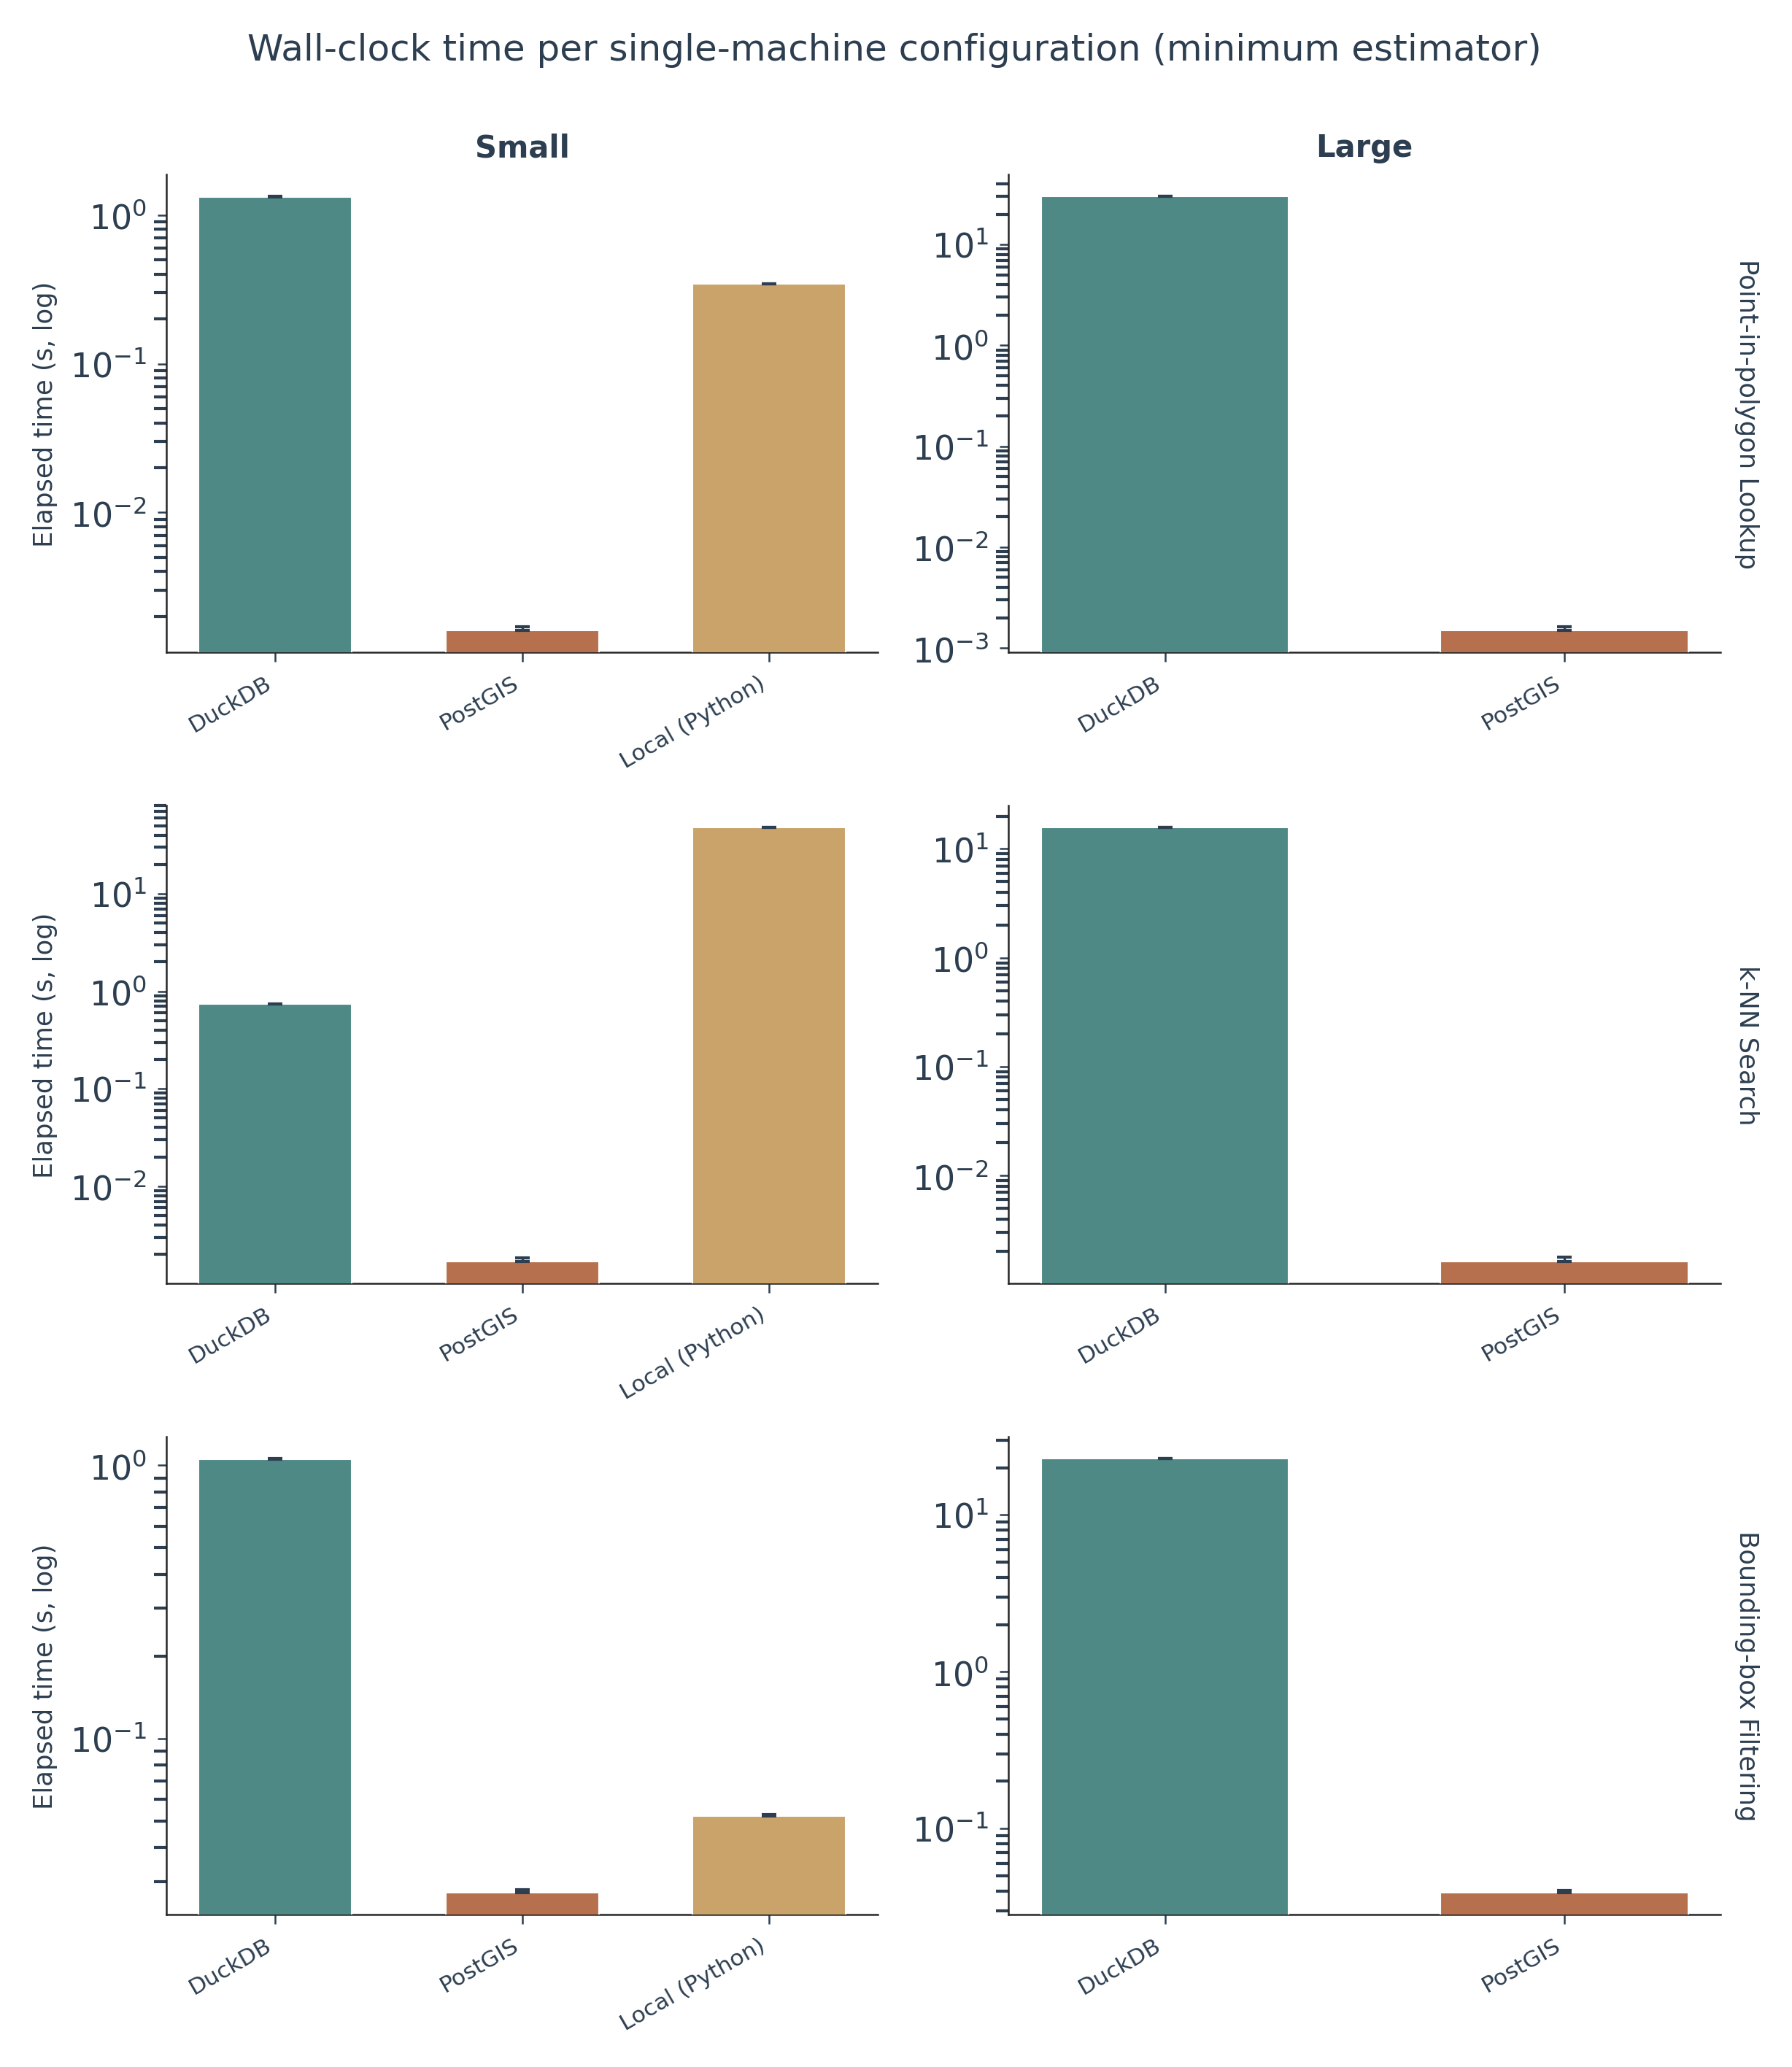
\includegraphics[width=0.95\textwidth]{Chapters/06-results/sub-chapters/figures/06-single-machine-wall-clock-time.png}
    \caption[Wall-clock time per single-machine configuration]{Wall-clock time of
    each single-machine configuration, in the same grid layout as the
    bytes-transferred figure: workload patterns in rows, size tiers in columns.
    Bar height is the minimum-estimator elapsed time on a logarithmic axis with
    bootstrap confidence-interval whiskers. Bar colour encodes configuration using
    the thesis palette.}
    \label{fig:single-machine-wall-clock-time}
\end{figure}

\subsection{Operational cost}
\label{results:single-machine-query-performance:operational-cost}

% TODO (prose): factual readout only of the operational-cost results, broken into
% the four cost terms. Refer to Figure~\ref{fig:single-machine-operational-cost}.
% No interpretation (-> Discussion).

\begin{figure}[H]
    \centering
    % WHAT IT SHOWS: stacked operational-cost bars, one bar per configuration,
    %   faceted by workload pattern. Each bar is stacked into the FOUR cost terms
    %   of the cost model: compute, storage, operations, and egress.
    % CAPTION MUST STATE: that cost is decomposed into the four model terms --
    %   compute, storage, operations, egress -- and name their source (the
    %   four-term cost model and unit-price table of the methodology). Note that a
    %   single-node engine reading from object storage draws all four terms,
    %   whereas the local-filesystem Shapefile path draws no operations/egress.
    % NOTE: the prior draft showed only two terms (compute + transfer); the real
    %   model is four-term -- see
    %   Section~\ref{research-design-and-methodology:metrics-and-cost-model:cost-model}
    %   and the rates in Table~\ref{tab:cost-model-unit-prices}.
    % Leave the Shapefile-beyond-small and kNN-large slots as did-not-run-by-design.
    % DESCRIPTIVE ONLY: report the stacks; no interpretation (-> Discussion).
    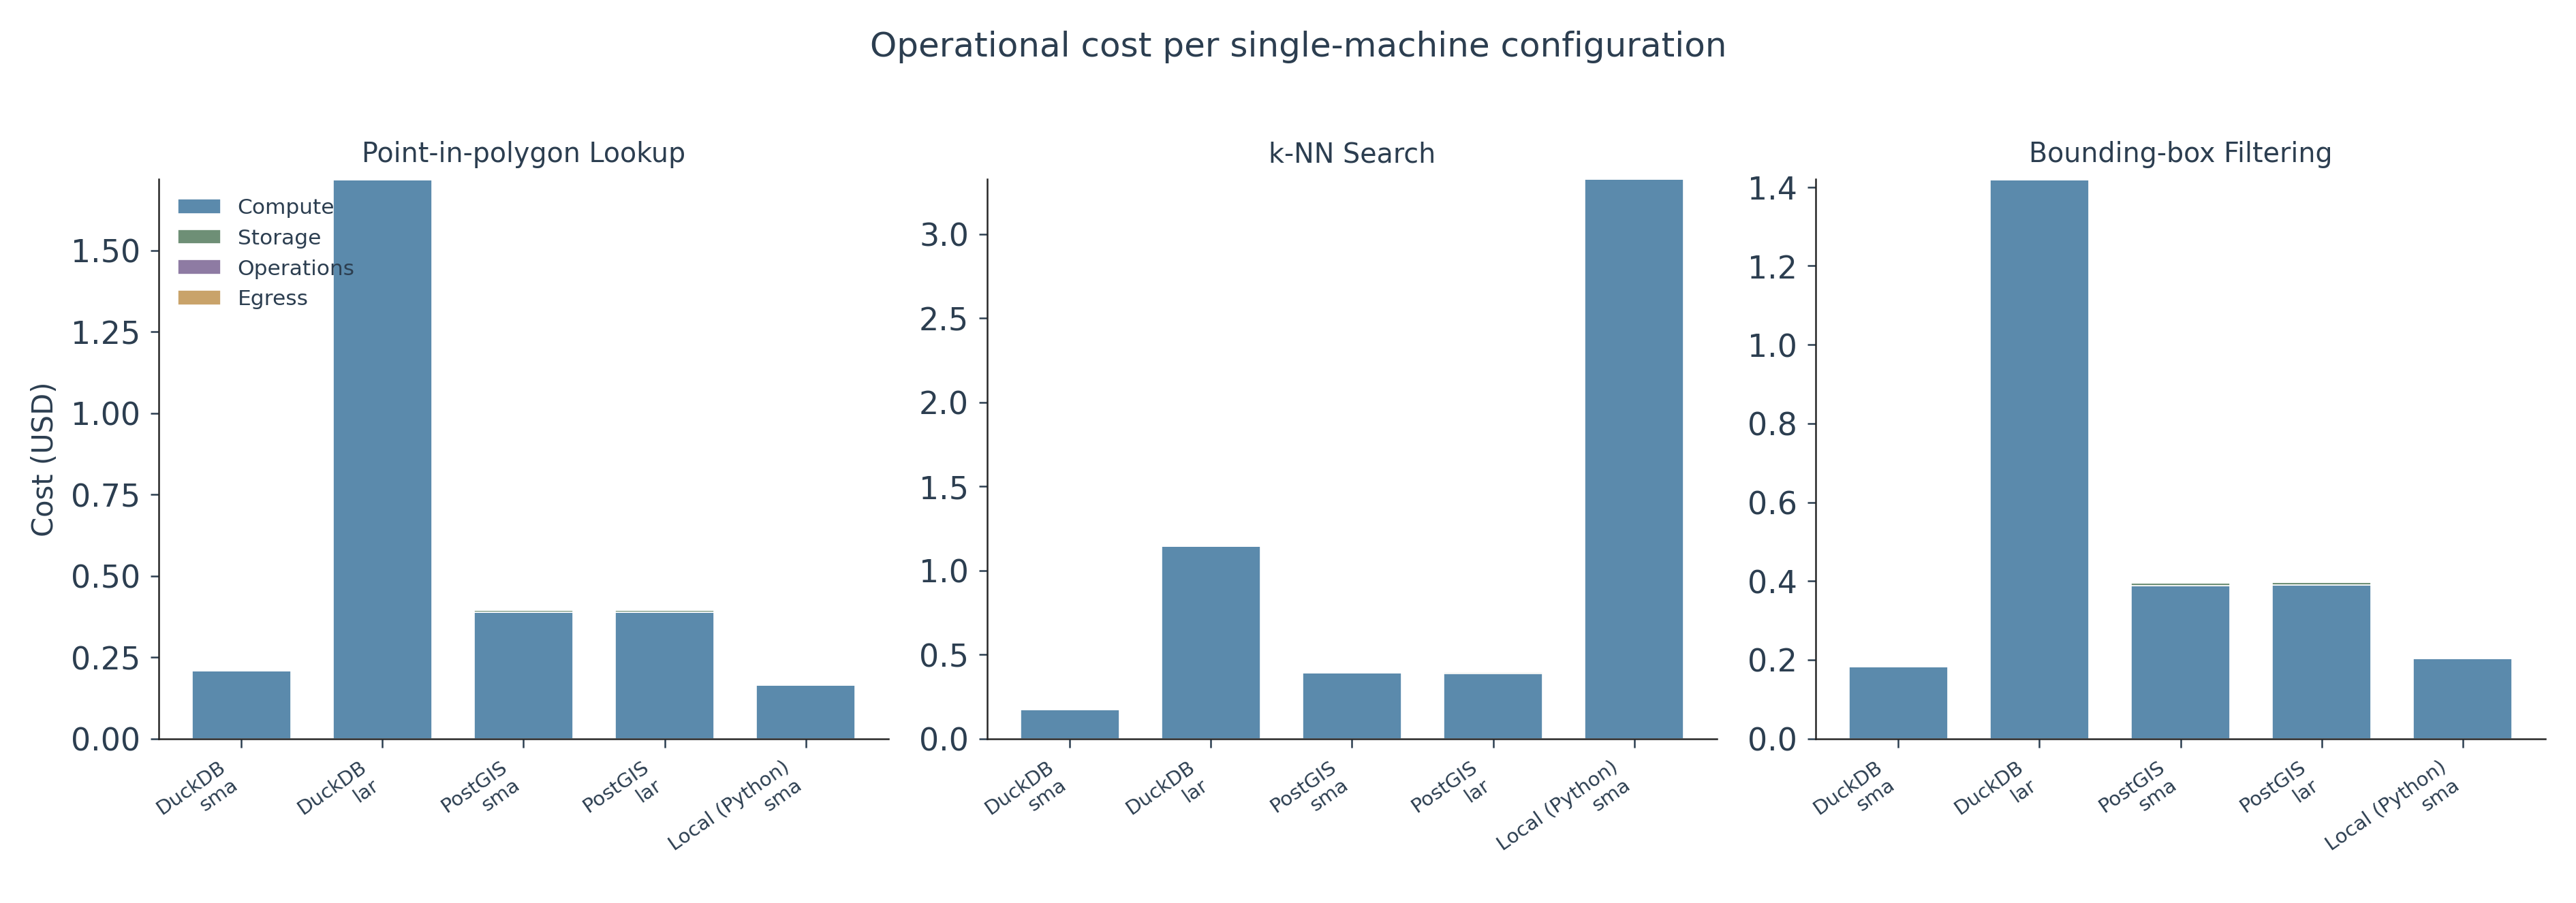
\includegraphics[width=0.9\textwidth]{Chapters/06-results/sub-chapters/figures/06-single-machine-operational-cost.png}
    \caption[Operational cost per single-machine configuration]{Operational cost
    of each single-machine configuration, faceted by workload pattern. Each bar is
    stacked into the four terms of the cost model -- compute, storage, operations,
    and egress -- whose definitions and unit prices are given in
    Section~\ref{research-design-and-methodology:metrics-and-cost-model:cost-model}
    and Table~\ref{tab:cost-model-unit-prices}. Term colour uses the thesis
    palette.}
    \label{fig:single-machine-operational-cost}
\end{figure}
